\section{Contributions}
\label{cap1:intro/contributions}
% \lipsum[1-3]
We present the three main contributions anticipated for this work.
\subsection*{Benchmark on Question Answering over Wikidata}
After a bibliographic revision, we will define a benchmark as a combination of three 
components: a baseline system, a set of metrics to compare with the baseline, and one or 
more datasets with which to conduct experiments.

The baseline consists of one of the Neural Machine Translation systems described by 
Yin et al.~\cite{nmt:nl-to-sparql-Yin19}. From the eight models that were compared in this work, 
the ConvS2S model~\cite{nmt:convS2S-GehringAGYD17} 
significantly outperforms all the other models . Following these results, a baseline QAS is 
implemented using the Fairseq library~\cite{nmt:fairseq-OttEBFGNGA19}, which includes a ConvS2S implementation over 
Pytorch\footnote{\url{https://pytorch.org/}} ready to use for training and translation. The model is trained using the same 
settings described by Yin et al.

The primary dataset used is the \LCQuADtwo{} dataset, which contains around $30,000$ 
questions over Wikidata~\cite{dataset:lcquad2-DubeyBA019}. A quality check is performed over this dataset, where cases 
that contain either invalid questions or invalid \SPARQL{} queries are filtered. The \DBNQA{} 
dataset~\cite{dataset:dbnqa-hartmann-marx-soru-2018} is considered as well, where a mapping process is applied to obtain queries over 
Wikidata. The queries that cannot be mapped are ignored. The Question Answering over 
Linked Data (QALD)~\cite{qa:qald-Lopezetal2013} dataset is also used as part of this benchmark. In particular, the 
150 questions included in \QALDseven{}~\cite{dataset:qald7-UsbeckNHKRN17} that can be answered over Wikidata are considered. 
Besides these datasets, we build a new dataset of 100 questions over Wikidata. Only \LCQuADtwo{} 
and the mapped version of \DBNQA{} are used for training and validation. The other 
datasets are used only for testing purposes. All datasets are arranged to follow a common 
format, which will permit an easy evaluation of every subtask performed for the proposed 
Question Answering system (Entity Linking, Query Template Generation, Slot Filling) along 
with the main task (Question Answering over Knowledge Graphs).

The metrics used for comparing systems are based on the ones used for comparing Neural 
Machine Translation systems and the ones found on the QALD benchmark. The first set of 
metrics includes the BLEU score, Perplexity, and Accuracy by comparing an exact match on 
the \SPARQL{} query. On the other hand, the QALD benchmark uses Precision, Recall, and F1-score 
over the answers obtained when executing the output \SPARQL{} query. Additionally, 
we propose a fine-grained analysis over each case where predicted queries are evaluated with 
respect to the following components: correct entities, correct slots, and correct query 
templates.

\subsection*{Question Answering system over Wikidata}
\label{cap1:intro/contributions/qaWikidata}

The main contribution of this work is a Question Answering system that translates 
natural language questions in English to \SPARQL{} queries executable on Wikidata endpoints. See an
example of an expected \SPARQL{} query in Figure~\ref{fig:introQAexample}. The implemention of this 
system is divided into the construction of three modules: a Query Template generator, 
an Entity Linking system, and an intermediate Slot Filling system. 

\begin{figure}[!h]
    \centering
    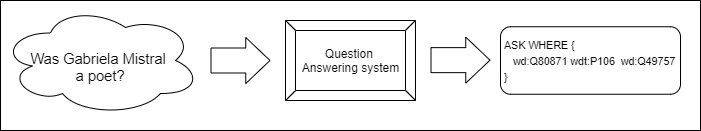
\includegraphics[scale=.5]{imagenes/1_intro/introQuestionAnsweringExample.png}
    \caption{Expected \SPARQL{} query example from a KGQA system.}
    \label{fig:introQAexample}
\end{figure}

The Query Template generator produces incomplete \SPARQL{} queries (which we call 
Query Templates) that contain \dquotesit{placeholders} in the position where entities are 
supposed to be (e.g. placeholders \texttt{<sbj\_1>} and \texttt{<obj\_1>} instead of entities 
\texttt{Q80871} and \texttt{Q49757} of the query shown in Figure~\ref{fig:introQAexample}). 
This module is built using the same model used to implement the baseline QAS. 
However, the training data is adapted to generate Query Templates instead of the complete 
query. This is achieved by removing the entities from the output \SPARQL{} queries included 
in the selected datasets such that the entities can rather be found by Entity Linking.

The role of the Entity Linking module is to recognize the relevant entities contained
in each question (e.g. identify that concepts \dquotesit{Gabriela Mistral} and \dquotesit{poet}
corresponds to the entities \texttt{Q80871} and \texttt{Q49757} in Figure~\ref{fig:introQAexample}) 
that are used to fill the Query Template. We implement various entity retrieval systems using 
one or more of the existing Entity 
Linking systems that have APIs available. The first variant is to use each EL system individually, 
which includes DBpedia Spotlight~\cite{EL:dbpedia-spotlight-MendesJGB11}, AIDA~\cite{EL:aida-tool-YosefHBSW11}, 
TAGME~\cite{EL:tagme-FerraginaS10}, and OpenTapioca~\cite{EL:opentapioca-Delpeuch19}. 
All of these systems, except for OpenTapioca, only work for DBpedia; therefore an 
extra mapping layer is implemented to map DBpedia entities to Wikidata entities. Two ensemble 
EL approaches are then proposed: one that prioritizes systems with higher Precision 
and another that implements a voting mechanism. We keep the variant that performs best 
according to the experiments that are explained in the \textit{Experimental results} subsection.

Additionally, a Slot Filling module is built by combining a Sequence Tagger model of the Flair 
library~\cite{seqlab:flair-AkbikBBRSV19} and a filling algorithm proposed in this work. Training 
the Sequence Tagger model requires building training data based on the selected datasets. 
Intuitively speaking, a Query Template may have multiple slots and multiple entities, where the 
Slot Filling module decides which entity should fill which slot (e.g. to infer that the concept 
\dquotesit{Gabriela Mistral} corresponds to the placeholder \texttt{<sbj\_1>}, therefore the 
entity \texttt{Q80871} should replace the occurences of \texttt{<sbj\_1>} in the Query Template).

\subsection*{Experimental results}
\label{cap1:intro/contributions/expResults}
We conduct several experiments for validating each implemented module (Entity Linking, 
Slot Filling, and Query Template Generation) along with experiments over the defined 
benchmark for the end-to-end Question Answering process.

The Entity Linking systems are compared using Precision, Recall, and F1-score on the 
entities for each case on the dataset used for training. Testing is conducted over \QALDseven{} and 
our proposed dataset. The slot filling system is validated using Precision, Recall, and F1-score 
over the identified BIO labels (a common tagging format for sequence labeling tasks) over 
\LCQuADtwo{} and the mapped \DBNQA{} dataset. The query generator system is validated 
using BLEU score, Perplexity, and Accuracy over \LCQuADtwo{} and the mapped \DBNQA{} 
dataset. When training the query generator system, many split methods are tested according 
to the methodology proposed by Finegan-Dollak et al.~\cite{semPar:txt-to-sql-RadevKZZFRS18} for Text-to-SQL systems. 
The end-to-end Question Answering system is tested over all the datasets using the metrics 
described in the \textit{Benchmark on Question Answering over Wikidata} subsection.